\section{A Step-by-step Guide to Running DPA on the example AES Implementation}

In this section we provide a step-by-step guide to attack the example AES included with FOBOS. We assume that the FOBOS software is installed in the \$fobos directory.
We also assume that Python is installed.

To run DPA attack on the AES implementation provided, follow these steps:
\begin{enumerate}
\item \textbf{Program the control board}
  \begin{enumerate}
  \item Create a new project using Xilinx ISE. In the New Project wizard set the Project Settings as in Fig~\ref{fig:ctrl-design-properties}.
  		\begin{figure}[H]
		\begin{center}
		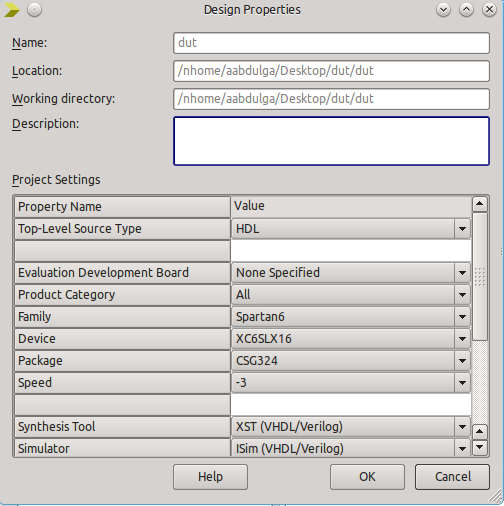
\includegraphics[scale=0.6]{figures/ctrl-design-properties}
		\caption{\label{fig:ctrl-design-properties}FOBOS Controller Desgin Properties}
		\end{center}
		\vspace{-1ex}
		\end{figure}
  \item From the Project menu select Add Source... and add all files from \texttt{\$fobos/sources/common}.
  \item Repeat the previous process to add all files from \texttt{\$fobos/sources/vhdl/control} (add all files except \texttt{Nexys3.ucf}) (See Fig~\ref{fig:ctrl-add-sources}).
		\begin{figure}[H]
		\begin{center}
		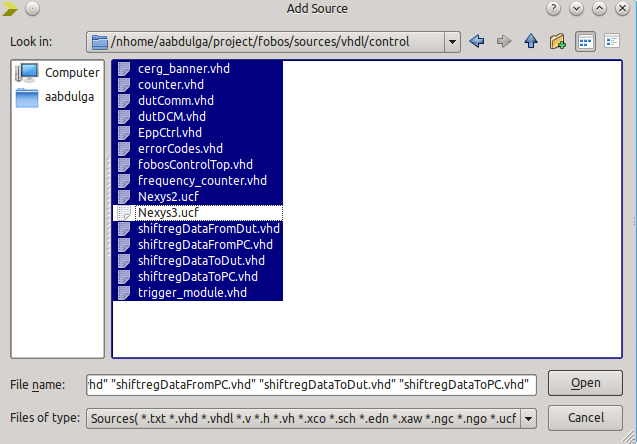
\includegraphics[scale=0.6]{figures/ctrl-add-sources}
		\caption{\label{fig:ctrl-add-sources}Adding Source Files to FOBOS Controller}
		\end{center} 
		\vspace{-1ex}
		\end{figure}
  \item Set the \texttt{fobosControlTopLevel} module as the top-level module for this project (See Fig~\ref{fig:ctrl-set-top-level}).
		\begin{figure}[H]
		\begin{center}
		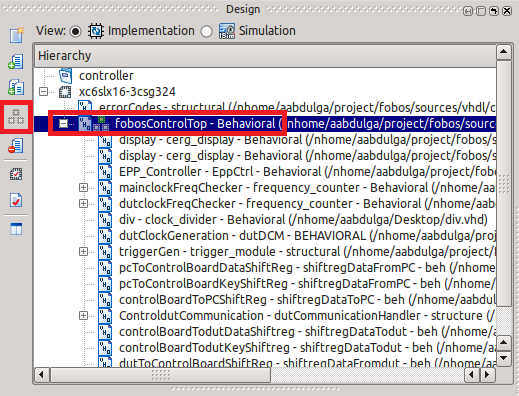
\includegraphics[scale=0.6]{figures/ctrl-set-top-level}
		\caption{\label{fig:ctrl-set-top-level}Setting Top-level Module}
		\end{center} 
		\vspace{-1ex}
		\end{figure}
  \item Generate the programming bit file for the control board by clicking "Generate Programming File" in the Processes window.
  \item Program the control board using Xilinx Impact. In the Processes window, click Configure Target Device (See Fig~\ref{fig:ctrl-run-impact}).
		\begin{figure}[H]
		\begin{center}
		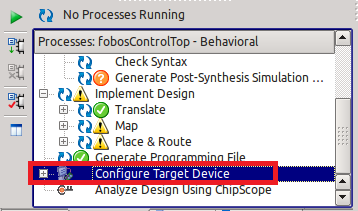
\includegraphics[scale=0.6]{figures/ctrl-run-impact}
		\caption{\label{fig:ctrl-run-impact}}
		\end{center}
		\vspace{-1ex}
		\end{figure}
  \item In the Impact window, click "Boundary Scan" then form the File menu, click "Initialize Chain" and assign the bit file to the FPGA. Now you may right-click the FPGA and click "Program".
		\begin{figure}[H]
		\begin{center}
		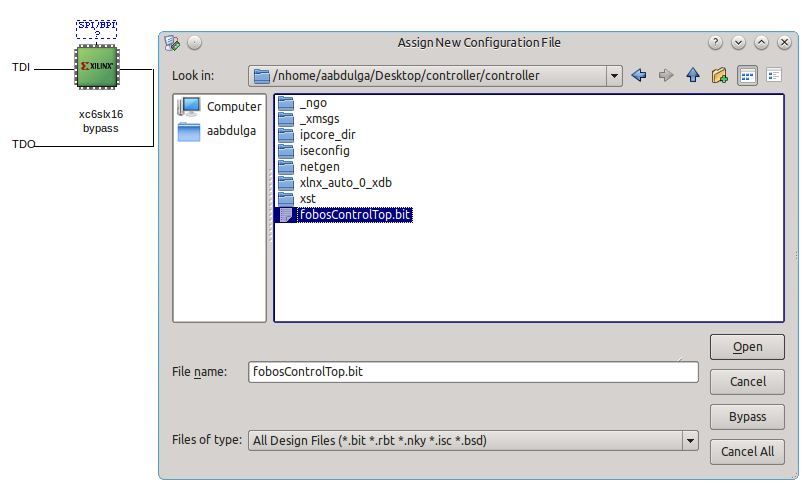
\includegraphics[scale=0.6]{figures/ctrl-program}
		\caption{\label{fig:ctrl-program}Progrmamming Control Board}
		\end{center}
		\vspace{-1ex}
		\end{figure}
  \end{enumerate}
\item \textbf{Program the victim board (DUT)}
  \begin{enumerate}
  \item Create a new project using Xilinx ISE. In the New Project wizard set the Project Settings as in Fig~\ref{fig:dut-design-properties}.
		\begin{figure}[H]
		\begin{center}
		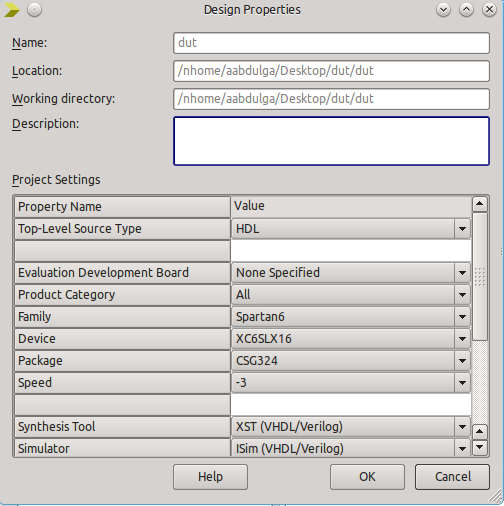
\includegraphics[scale=0.6]{figures/dut-design-properties}
		\caption{\label{fig:dut-design-properties}DUT Design Properties}
		\end{center}
		\vspace{-1ex}
		\end{figure}
  \item From the Project menu select Add Source... and add all files from \texttt{\$fobos/sources/common}.
  \item Repeat the previous process to add all files from \texttt{\$fobos/sources/vhdl/DUT} (add all files except \texttt{Nexys.*}) and all files from \texttt{\$fobos/examples/AES-128/vhdl}  (See Fig~\ref{fig:dut-add-sources}).
		\begin{figure}[H]
		\begin{center}
		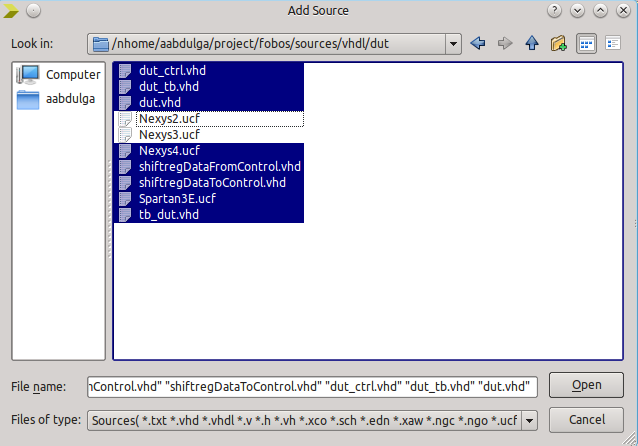
\includegraphics[scale=0.6]{figures/dut-add-sources}
		\caption{\label{fig:dut-add-sources}DUT Add Sources}
		\end{center}
		\vspace{-1ex}
		\end{figure}
  \item Make sure to not use block RAMs in the implementation. .
     \begin{enumerate}
	\item Make sure to select the "Implementation" view.
        \item Right-click the Synthesize-XST processes.
	\item In the Preocess Properties window, select HDL Options and select "Distributed" for the RAM Style property (See Fig~\ref{fig:dut-ram-style}).
	\item Click OK.
		\begin{figure}[H]
		\begin{center}
		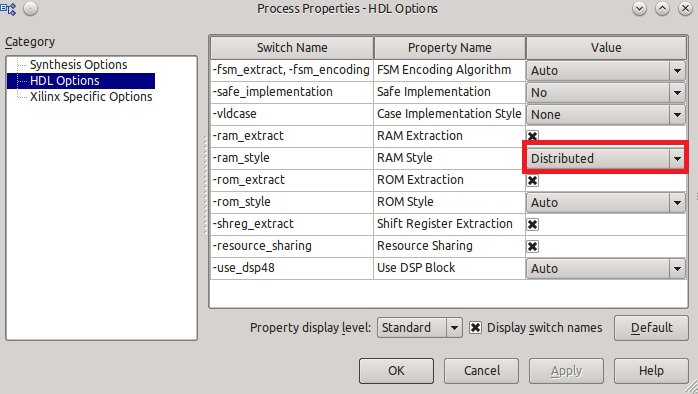
\includegraphics[scale=0.6]{figures/dut-ram-style}
		\caption{\label{fig:dut-ram-style}DUT RAM Style}
		\end{center}
		\vspace{-3ex}
		\end{figure}
     \end{enumerate}
  \item Set the \texttt{dutTopLevel} as the top-level module in this project.
		\begin{figure}[H]
		\begin{center}
		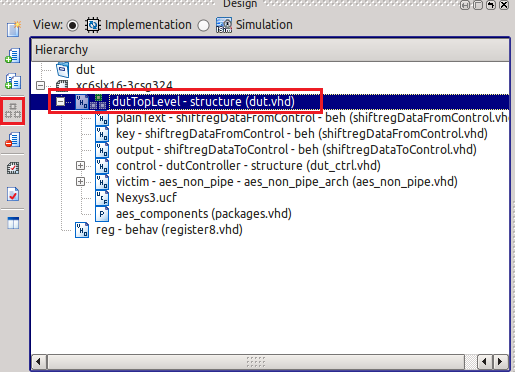
\includegraphics[scale=0.6]{figures/dut-set-top-level}
		\caption{\label{fig:dut-set-top-level}Set DUT Top-level}
		\end{center}
		\vspace{-3ex}
		\end{figure}
  \item Generate the programming bit file for the DUT by clicking "Generate Programming File" in the Processes window.
  \item Program the DUT using Xilinx Impact. In the Processes window, click Configure Target Device (See Fig~\ref{fig:dut-run-impact}).
		\begin{figure}[H]
		\begin{center}
		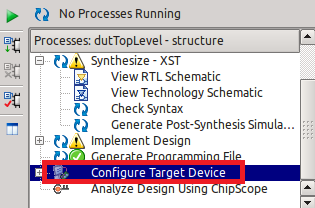
\includegraphics[scale=0.6]{figures/dut-run-impact}
		\caption{\label{fig:dut-run-impact}}
		\end{center}
		\vspace{-3ex}
		\end{figure}
  \item In the Impact window, click "Boundary Scan" then form the File menu, click "Initialize Chain" and assign the bit file to the FPGA. Now you may right-click the FPGA and click "Program".
		\begin{figure}[H]
		\begin{center}
		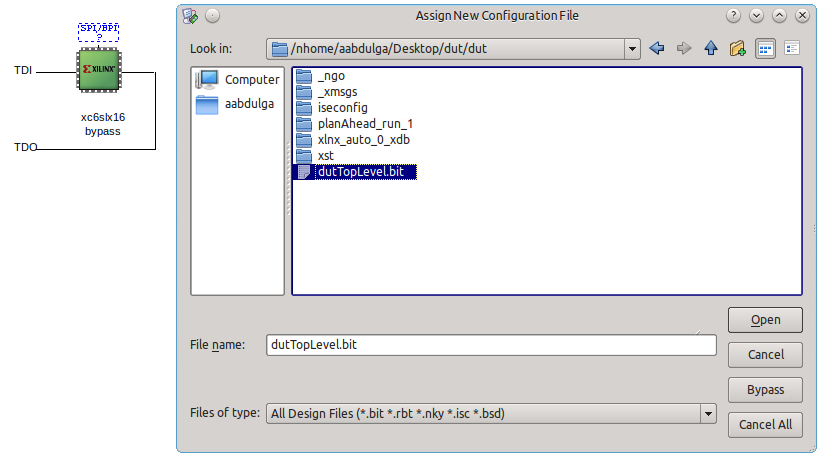
\includegraphics[scale=0.6]{figures/dut-program}
		\caption{\label{fig:dut-program}Progrmamming DUT}
		\end{center}
		\vspace{-3ex}
		\end{figure}
  \end{enumerate}
\item \textbf{Connect hardware}
  \begin{enumerate}
  \item Connect control board to power and ground.
  \item Connect control board tirgger output to channel 2 on the oscilloscope.
  \item Connect the control board to the DUT using the bridge connector.
  \item Connect the control board to the PC running the FOBOS software using USB.
  \item Connect clock generator to the bridge connector. Set the clock generator clock to 600 KHz.
  \item Connect the current probe to channel 1 on the oscilloscope.
  \item Connect the current probe to the DUT's ground.
  \item Connect DUT to power making sure that the current probe is measuring the current.
  \item Connect DUT to power supply ground.
  \end{enumerate}
\item \textbf{Run FOBOS Capture}
  \begin{enumerate}
  \item In console type:
    \texttt{cd \$fobos/bin}
  \item Edit the texttt{\$fobos/config/acquisitionConfig.txt} fil to look like the following (Make sure to set OSCILLOSCOPE\_IP and OSCILLOSCOPE\_PORT to correct values) :
    

    \begin{figure}[H]
    \begin{Verbatim}[frame=single]
# =============================================
# Global Settings
# =============================================
MEASUREMENT_FORMAT = dat # Default => dat
LOGGING = INFO # INFO|DEBUG
# =============================================
# Control Board Settings
# =============================================
CONTROL_BOARD = Nexys2
VICTIM_RESET = 11
TIME_OUT = 50000
TRIGGER_WAIT_CYCLES = 1 #@VICTIM CLOCK must be >0
TRIGGER_LENGTH_CYCLES = 1 #@VICTIM CLOCK
# =============================================
# Test Data Generation Settings
# =============================================
PLAINTEXT_GENERATION = RANDOM # USER | RANDOM
DATA_FILE     = plaintexts.txt
KEY_GENERATION = RANDOM # USER | RANDOM 
KEY_FILE      = keys.txt
INPUT_FORMAT  = hex # Default => hex
OUTPUT_FORMAT = hex # Default => hex
NUMBER_OF_ENCRYPTIONS_PER_TRACE = 1
BLOCK_SIZE = 16 # In Bytes
KEY_SIZE = 16 # In Bytes
# =============================================
# FOBOS Capture Settings
# =============================================
DUMMY_RUN = NO  #YES/NO
NUMBER_OF_TRACES = 20
####################################################
######## Signal Alignment Module Parameters ########
####################################################
CAPTURE_MODE = SINGLE # MULTI|SINGLE
TRIGGER_THRESHOLD = 1.0
# =============================================
# FOBOS Oscilloscope Settings
# ============================================
# INTIALIZATION OPTIONS
OSCILLOSCOPE = AGILENT #AGILENT|OPENADC
OSCILLOSCOPE_IP = 192.168.0.10
OSCILLOSCOPE_PORT = 5025
AUTOSCALE = NO   # YES|NO    
IMPEDANCE = FIFTY #FIFTY|ONEMEG
# VOLTAGE AND TIME RANGE OPTIONS        
CHANNEL1_RANGE = 0.12V
CHANNEL2_RANGE = 6V
CHANNEL3_RANGE = OFF # ON|OFF|voltage range
CHANNEL4_RANGE = OFF # ON|OFF|voltage range
TIME_RANGE = 0.000028
TIMEBASE_REF = LEFT    
# TRIGGER OPTIONS
TRIGGER_SOURCE =  CHANNEL2
TRIGGER_MODE =  EDGE   
TRIGGER_SWEEP = NORM
TRIGGER_LEVEL = 1
TRIGGER_SLOPE = POSITIVE
# ACQUIRE OPTIONS
ACQUIRE_TYPE = NORM # NORM|PEAK|HRES|AVER
ACQUIRE_MODE = RTIM   # RTIM | ETIM| SEG
      \end{Verbatim}
      \caption{\label{fig:fobos:acqconf}Snippet of acquisitionConfig.txt}
      \end{figure}
      
      \item Run the acquisition script as follows: \texttt{python dataAcqusition.py}
      
  \end{enumerate}
 \item \textbf{Load your hypothetical power data.}
  \begin{enumerate}
   \item Copy the aes\_hw.py script from \$fobos/examples/AES-128/powermodel/ to \$fobos/FOBOSWorkspace/testing/\$attempt/output.
   \item Generte your hypothetical data. Run \texttt{python3 aes\_hw.py}
   \item Copy the hypothetical data files to the \$fobos/data/ directory.
  \end{enumerate}

\item \textbf{Run FOBOS Analysis.}
  \begin{enumerate}
   \item Edit the configuration files in the \$fobos/config directory as follows:
   
   
   \textbf{compressionParams.txt}
   \begin{figure}[H]
	\begin{Verbatim}[frame=single]
####################################################
######## Compression Module Parameters #############
####################################################
COMPRESSION_LENGTH = 10
COMPRESSION_TYPE = MEAN # MAX|MIN|MEAN
	\end{Verbatim}
	\caption{\label{fig:fobos:paramsa}Snippet Compression Parameters}
	\end{figure}
	
  
   \textbf{dataAnalysisParams.txt}
   \begin{figure}[H]
	\begin{Verbatim}[frame=single]
WORK_DIR = FOBOSAnalysis
MEASUREMENT_WORK_DIR = FOBOSWorkspace
TAG = counter
	\end{Verbatim}
	\caption{\label{fig:fobos:paramanalysis}Snippet Data Analysis Parameters}
	\end{figure}
	
   
   \textbf{dataAnalysisParams.txt}
   \begin{figure}[H]
	\begin{Verbatim}[frame=single]
####################################################
######## Post Processing Flow ######################
####################################################
SAMPLE_SPACE_DISPOSITION = 2 # 1-3|NO
COMPRESS_DATA = 3 #1-3|NO
TRACE_EXPUNGE = 1 #1-3|NO 
TRACE_EXPUNGE_PARAMS = VAR-0.0000110:0.0000139 #STD|VAR-BELOW:ABOVE|NO
	\end{Verbatim}
	\caption{\label{fig:fobos:parampsotproc}Snippet Post Processing Parameters}
	\end{figure}
	
   \textbf{sampleSpaceDispParams.txt}
   \begin{figure}[H]
	\begin{Verbatim}[frame=single]
####################################################
#### Sample Space Disposition Module Parameters ####
####################################################
SAMPLE_WINDOW_SIZE = 2000
SAMPLE_WINDOW_START = 100 
	\end{Verbatim}
	\caption{\label{fig:fobos:paramdisp}Snippet Sample Space Disposition Parameters}
	\end{figure}
	
    
   \textbf{signalAlignmentParams.txt}
   \begin{figure}[H]
	\begin{Verbatim}[frame=single]
####################################################
######## Signal Alignment Module Parameters ########
####################################################
CAPTURE_MODE = SINGLE # MULTI|SINGLE
TRIGGER_THRESHOLD = 1.0
	\end{Verbatim}
	\caption{\label{fig:fobos:paramalingn}Snippet Signal Alignment Parameters}
	\end{figure}
   
   \textbf{traceExpungeParams.txt}
   \begin{figure}[H]
	\begin{Verbatim}[frame=single]
####################################################
######## Trace Expunge Module Parameters ###########
#################################################### 
TRACE_EXPUNGE_PARAMS = VAR:0.0004:0.00045 #STD|VAR:BELOW:ABOVE|NO
	\end{Verbatim}
	\caption{\label{fig:fobos:paramexpunge}Snippet Trace Expunge Parameters}
	\end{figure}
    \item Run the Data Analysis script: \texttt{python dataAnalysis.py}
    \item Check the analysis output files in \$fobos/FOBOSWorkspace/testing/\$attempt/analysis.
  \end{enumerate}


\end{enumerate}
